\chapter{Particle Flow Calorimetry and Linear Collider Detectors}
\label{chap:reconstructionchain}

\chapterquote{I am fond of pigs.  Dogs look up to us.  Cats look down on us.  Pigs treat us as equals.}
{Winston Churchill}

\section{Particle Flow Calorimetry}

The premise of particle flow calorimetry is to measure the energy of individual particles in detector using the sub-detector that offers the best energy resolution.  For particle collider experiments, the biggest contrast to tradition calorimetry is that the energy of charged particles is measured using the curvature of the tracks they produce in the tracker instead of measuring their energy in calorimeters.  The energy resolution for these charged particles is significantly better when using the particle flow approach to calorimetry, which leads to exceptionally good jet energy resolutions that can be used for characterising multi-jet final states in physics processes of interest at the linear collider experiment.  Furthermore, these energy resolutions are highly beneficial for quantifying those final states involving charged leptons and missing momentum, due to the presence of neutrinos.

\begin{figure}
\centering
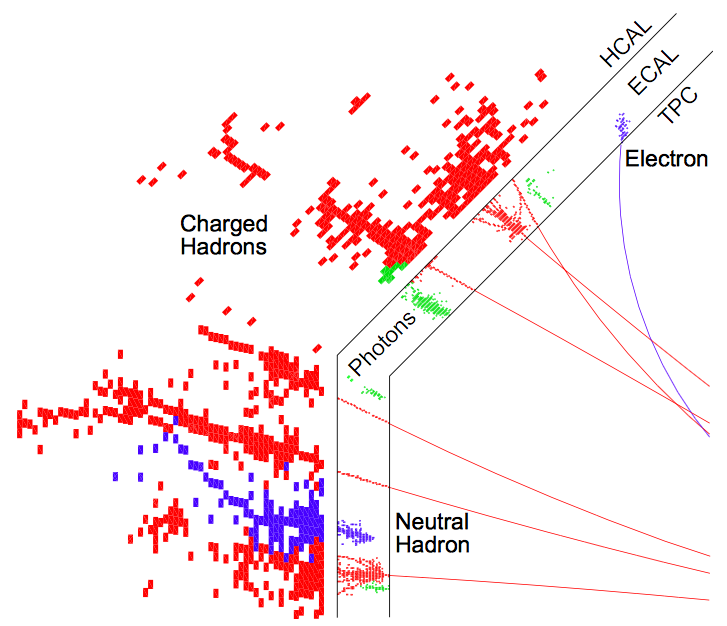
\includegraphics[width=0.5\textwidth]{LCDetectorsAndPFlow/Plots/Pictures/PFlow.png}
\caption[A typical simulated 250 GeV jet in the CLIC\_ILD detector, with labels identifying constituent particles.  Image taken from  \cite{arXiv:1209.4039}.]{A typical simulated 250 GeV jet in the CLIC\_ILD detector, with labels identifying constituent particles.  Image taken from  \cite{arXiv:1209.4039}.}
\label{fig:particleflowpic}
\end{figure} 

Particle flow calorimetry is challenging to put into practice as it requires a precise reconstruction for all long-lived particles within a detector.  Charged particles have their energy measurements taken from the curvature of the track they transverse, but they also produce calorimetric energy deposits, as shown in figure \ref{fig:particleflowpic}, and if both energy measurements are included the energy of the charged particle will be double counted.  Therefore, the precise reconstruction has to associate charged particle tracks to their corresponding calorimetric energy deposits.  This can only be realised by using calorimeters with fine segmentation so that it is possible to resolve individual particle showers within them.  This is the basis for the design of the linear collider calorimeters.  While double counting of energy of charged particles is possible, it is also possible to omit the energy measurements of neutral particles.  This occurs if a neutral particle calorimetric energy deposit, which is the only energy measurement produced for a neutral particle, is incorrectly associated to a track.  In such a case the calorimetric energy deposit will not be used as the reconstruction believes the energy is from a charged particle and so will come from the track and the neutral hadron energy will be lost.  These two effects form the confusion contribution to the jet energy resolution, which acts to degrade the energy resolution of a particle flow calorimetry based detector.  

\begin{table}[h!]
\centering
\begin{tabular}{ l l l l l}
\hline
Jet  & Detector & Energy & Energy & Jet Energy \\
Component &  & Fraction & Resolution & Resolution Contribution \\
\hline
Charged & Tracker & $\sim 0.6 E_{j}$ & $10^{-4} \times E_{X^{\pm}}^{2}$ & $< 3.6 \times 10^{-5} \times E_{j}^{2}$ \\
Particles ($X^{\pm}$) & & & & \\
Photons & ECal & $\sim 0.3 E_{j}$ & $0.15 \times \sqrt{E_{\gamma}}$ & $0.08 \times \sqrt{E_{j}}$ \\
($\gamma$) & & & & \\
Neutral & HCal &$\sim 0.1 E_{j}$ & $0.55 \times \sqrt{E_{X^{0}}}$ & $0.17 \times \sqrt{E_{j}}$ \\
Hadrons ($X^{0}$) & & & & \\
\hline
\end{tabular}
\caption[The approximate fractions, energy resolutions and jet energy resolution contributions made by charged particles ($X^{\pm}$), photons ($\gamma$) and neutral hadrons ($X^{0}$).  Table taken from \cite{arXiv:0907.3577}.]{The approximate fractions, energy resolutions and jet energy resolution contributions made by charged particles ($X^{\pm}$), photons ($\gamma$) and neutral hadrons ($X^{0}$).  Table taken from \cite{arXiv:0907.3577}.}
\label{table:pflowjet}
\end{table}

The magnitude of the improvements offered by particle flow calorimetry can be explicitly seen when considering the different contributions to the measurement of jet energies, which is summarised in table \ref{table:pflowjet}.  After the decay of short lived particles approximately 60\% of the energy of a jet is carried in the form of charged particles, 30\% in the form of $\gamma$s and 10\% in the form of neutral hadrons.  A negligible amount of energy is also carried in the form of invisible energy i.e. neutrinos.  In the traditional calorimetric approach $\gamma$s are measured within the ECal, with an energy resolution of $\sim 0.15 \times \sqrt{E_{\gamma}}$, and the remaining particles are measured in the HCal, with an energy resolution of $\sim 0.55 \times \sqrt{E_{X}}$.  This gives contributions to the jet energy, $E_{j}$, resolution of $\frac{0.08}{\sqrt{E_{j}}}$ and $\frac{0.46}{\sqrt{E_{j}}}$ from $\gamma$s and other particles respectively.  These add in quadrature to give a total jet energy resolution of $\frac{0.47}{\sqrt{E_{j}}}$.  In the particle flow paradigm the energy of charged particles is measured in the tracker, which has such a good energy resolution that its contribution to the jet energy resolution is negligible.  Therefore, contributions to the jet energy resolutions only come from $\gamma$s and from neutral hadrons, which when added in quadrature give a total jet energy resolution of $\frac{0.19}{\sqrt{E_{j}}}$.  This jet energy resolution is significantly better than that offered by the traditional calorimetric approach, however, it must be emphasised that this is an upper limit on the performance as the effect of confusion will degrade the jet energy resolution.  By applying sophisticated pattern recognition algorithms this confusion can be minimised and exceptional performance achieved.  While numerous approximations have been made in the above calculation it is clear that particle flow calorimetry has the potential to revolutionise detector deign for high energy physics experiments.

\section{Linear Collider Detectors}

All detector concepts for the linear collider have been purposely built to make particle flow calorimetry possible.  While there are a number of different concepts that are under consideration for both the ILC and CLIC one of the most prominent, and the focus of this work, is the International Large Detector (ILD).  The ILD detector, shown in figure \ref{fig:ild} realises very high spatial resolution for all sub-detector systems thanks to its highly granular calorimeters and central tracking system, all of which is encompassed within a 3.5 T magnetic field.  When combined with sophisticated pattern recognition software provided by PandoraPFA, particle flow calorimetry can be realised and the jet energy resolution can reach the goal of $3.8 \%$ which is required to allow separation of hadronic decays from W and Z bosons.  Details on each of the various sub-detector systems for ILD will now be discussed.

\begin{figure}
\centering
\subfloat[]{\label{fig:ild1}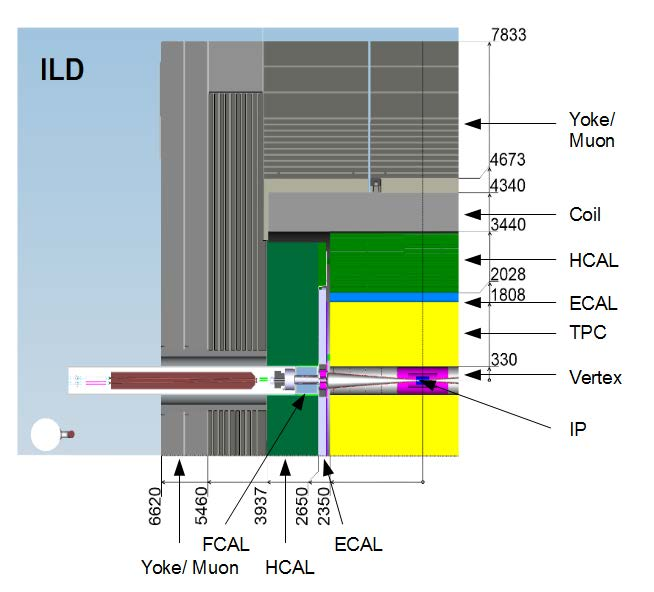
\includegraphics[width=0.5\textwidth]{LCDetectorsAndPFlow/Plots/Pictures/ILD.jpg}}
\subfloat[]{\label{fig:ild2}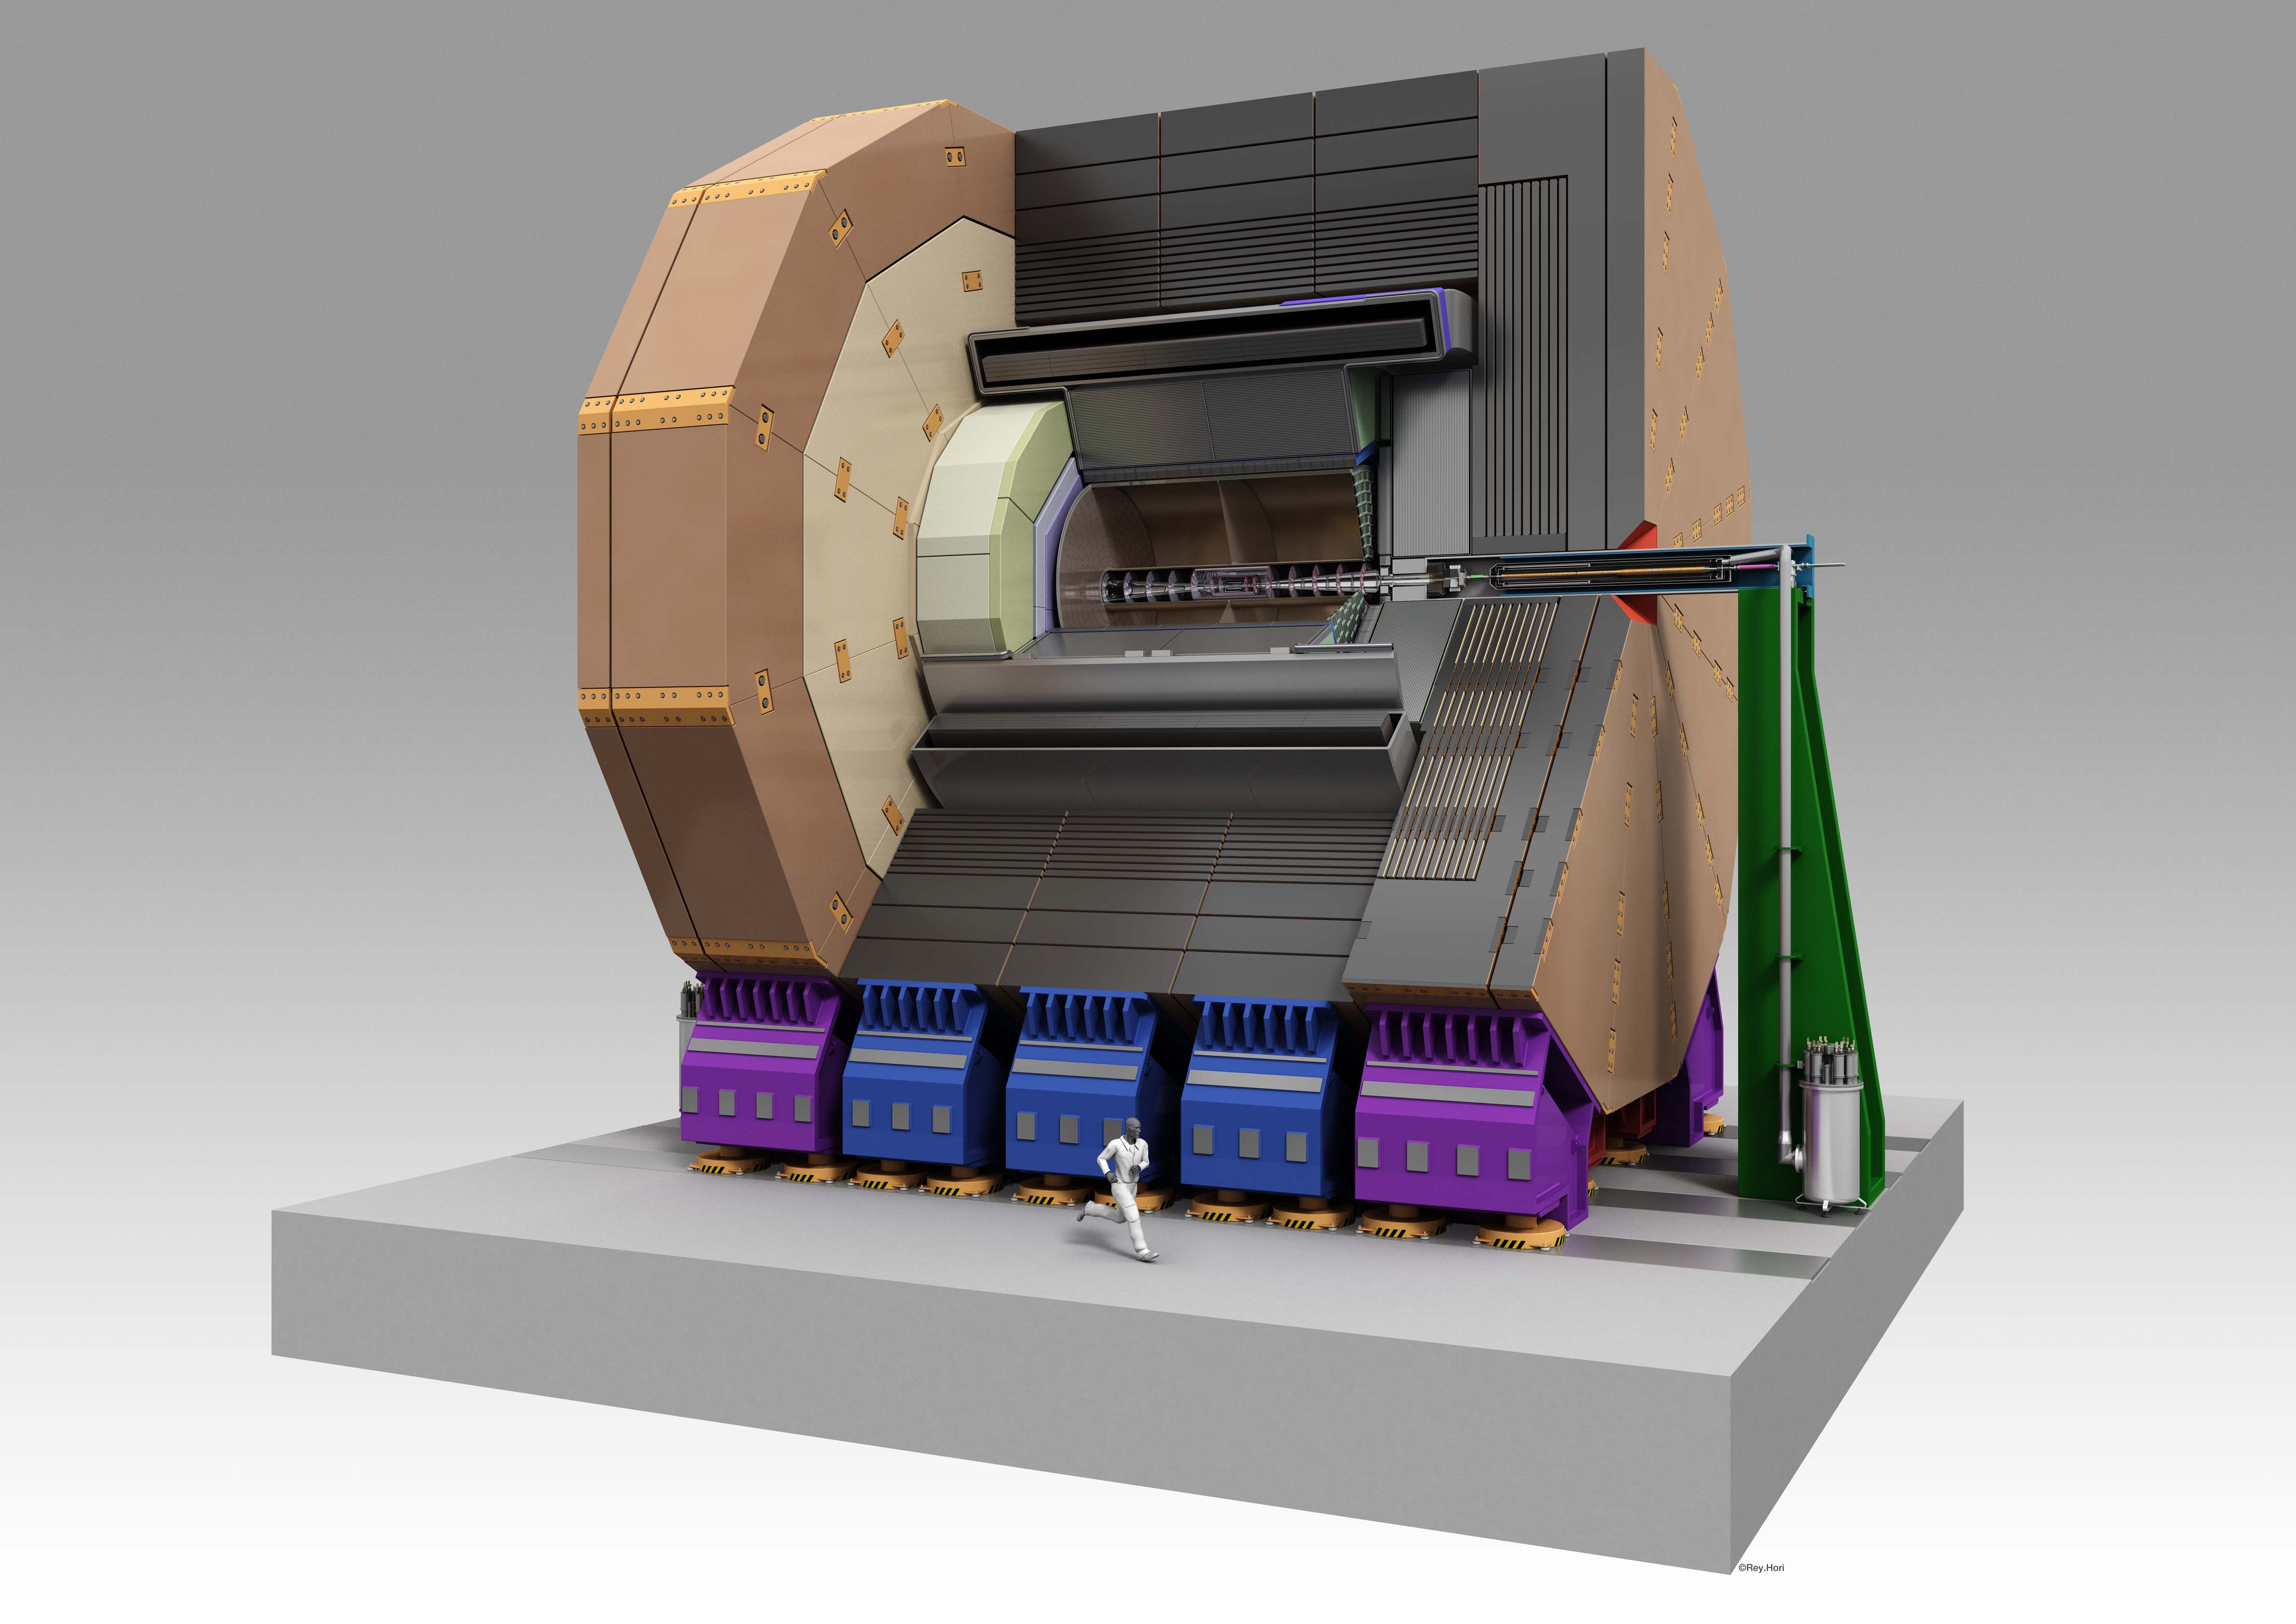
\includegraphics[width=0.5\textwidth]{LCDetectorsAndPFlow/Plots/Pictures/ILD_2.jpg}}
\caption[\protect\subref{fig:ild1} Quadrant view of the ILD detector concept.  The interaction point is in the lower right corner of the picture.  Dimensions are in mm.  \protect\subref{fig:ild2} View of the ILD detector concept.  Images taken from  \cite{Behnke:2013lya}.]{\protect\subref{fig:ild1} Quadrant view of the ILD detector concept.  The interaction point is in the lower right corner of the picture.  Dimensions are in mm.  \protect\subref{fig:ild2} View of the ILD detector concept.  Images taken from  \cite{Behnke:2013lya}.}
\label{fig:ild}
\end{figure} 

\subsection{Tracking System}
The tracking system for the ILD detector consist of a multi-layer pixel-vertex detector, which is surrounded by a system of silicon strip and pixel detectors.  These are purposed to give precise information about displaced vertices with respect to the impact point, which are crucial for the study of short lived particles such as the $D$ or $B$ mesons.  Outside of the vertex detector the central tracker of ILD, which is a Time Projection Chamber (TPC).  The TPC allows each charged particle track to be sampled at many space points giving precise information that can be used to extract the curvature of the track and the momentum of the charged particle transversing the track.  Finally, a further silicon strip detector surrounds the TPC to give an additional, high precision, space point to aid in the tracking performance. 

\subsubsection{Vertex System}
The main goal of the ILD vertex detector is to achieve a resolution on the impact parameter of charged particle tracks of $\sigma_{b} < 5 \oplus \frac{10}{p\text{sin}(\theta)^{3/2}} \mu$m.

\subsubsection{TPC}

\subsection{Electromagnetic Calorimeter}
A highly segmented electromagnetic sampling calorimeter (ECal) surrounds the ILD tracking system, which has been designed to make particle flow calorimetry a reality.  With that in mind the spatial resolution of particles showering within the calorimeter takes as much, if not more, precedence than the energy resolution of the detector.  

The primary goal of the ECal is to induce electromagnetic particles to shower within it and to record the energy deposited by those showers.  To that extent the ECal is constructed with tungsten as the absorber material.  As well as containing a large number of radiation lengths ($X_{0}$) per unit length tungsten also has a small Moli�re radius and a large ratio of the radiation length to the nuclear interaction length.  The small Moli�re radius will lead to compact electromagnetic showers and make the separation of nearby showers easier, while the large ratio of the radiation length to nuclear interaction length will lead to greater longitudinal separation between electromagnetic and hadronic showers.   

The nominal ILD ECal is a silicon tungsten sampling calorimeter, which contains 30 layers and uses square cells with side length 5 mm, however, a scintillator strip option is also under consideration.    

\subsection{Hadronic Calorimeter}
A hadronic calorimeter (HCal) surrounds the ECal and its primary goal is to measure particles showering hadronically.  The nominal ILD HCal is a scintillator steel sampling calorimeter, which contains 48 layers and uses square cells with side length 30 mm.      
 
\subsection{Forward Calorimetry}
A number of forward calorimeters are envisaged for the linear collider.  The primary purpose of these calorimeters is to extend the coverage of the detector towards 4\pi and to monitor the beam quality.  

\subsection{Muon Chamber}
Outside the HCal is the coil that generates the 3.5 T magnetic field and surrounding this is the iron yoke.  The purpose of this yoke is to return the magnetic flux from the extremely large magnetic field and to serve as a muon detector and a tail catcher for the calorimetry.  The yoke uses scintillator strip readout and for the simulations uses a $3\times3 \text{cm}^{2}$ cells.  This is in contrast to the ILD baseline, which plans to use 3 cm wide strips and 1 m long strips, however as the tail-catcher plays a minimal role in particle flow at ILC like energies this should have minimal impact.  

\subsection{CLIC ILD}

\section{PandoraPFA}

